\documentclass[onecolumn, draftclsnofoot,10pt, compsoc]{IEEEtran}
\usepackage{graphicx}
\usepackage{url}
\usepackage{svg} 
\usepackage{setspace} 
\usepackage{float}
\usepackage{longtable}
\usepackage{pgfgantt}
\usepackage{minted}
\usepackage{geometry}
\geometry{textheight=9.5in, textwidth=7in}


\def \subparagraph {.}

\usepackage{titlesec}
\usepackage{hyperref}

\titleclass{\threesection}{straight}[\subsection]
\titleclass{\foursection}{straight}[\subsection]

\newcounter{threesection}[subsubsection]
\newcounter{foursection}[threesection]

\renewcommand\thethreesection{\thesubsubsection.\arabic{threesection}}
\renewcommand\thefoursection{\thethreesection.\arabic{foursection}}

\renewcommand\theparagraph{\thethreesection.\arabic{paragraph}}
\renewcommand\theparagraph{\thefoursection.\arabic{paragraph}}

\titleformat{\threesection}
  {\normalfont\normalsize\bfseries}{\thethreesection}{1em}{}
\titlespacing*{\threesection}
{0pt}{3.25ex plus 1ex minus .2ex}{1.5ex plus .2ex}

\titleformat{\foursection}
  {\normalfont\normalsize\bfseries}{\thefoursection}{1em}{}
\titlespacing*{\foursection}
{0pt}{3.25ex plus 1ex minus .2ex}{1.5ex plus .2ex}


\makeatletter
\renewcommand\paragraph{\@startsection{paragraph}{6}{\z@}%
  {3.25ex \@plus1ex \@minus.2ex}%
  {-1em}%
  {\normalfont\normalsize\bfseries}}
\renewcommand\subparagraph{\@startsection{subparagraph}{7}{\parindent}%
  {3.25ex \@plus1ex \@minus .2ex}%
  {-1em}%
  {\normalfont\normalsize\bfseries}}
\def\toclevel@threesection{4}
\def\toclevel@foursection{5}
\def\toclevel@paragraph{6}
\def\toclevel@paragraph{7}
\def\l@threesection{\@dottedtocline{4}{7em}{4em}}
\def\l@foursection{\@dottedtocline{5}{10em}{5em}}
\def\l@paragraph{\@dottedtocline{6}{14em}{6em}}
\def\l@subparagraph{\@dottedtocline{7}{19em}{7em}}
\makeatother

\setcounter{secnumdepth}{4}
\setcounter{tocdepth}{4}
\setcounter{secnumdepth}{5}
\setcounter{tocdepth}{5}


% 1. Fill in these details
\def \CapstoneTeamName{			PolyVox}
\def \CapstoneTeamNumber{		66}
\def \GroupMemberOne{			Chris Bakkom}
\def \GroupMemberTwo{			Richard Cunard}
\def \GroupMemberThree{			Braxton Cuneo}
\def \CapstoneProjectName{		3D Virtual Reality Painting}
\def \CapstoneSponsorCompany{		EECS}
\def \CapstoneSponsorPersonOne{		Dr. Kirsten Winters}
\def \CapstoneSponsorPersonTwo{		Dr. Mike Bailey}
\def \CapstoneSponsorPersonTwo{		Dr. Mike Bailey}

% 2. Uncomment the appropriate line below so that the document type works
\def \DocType{		%Problem Statement
				%Requirements Document
				%Technology Review
				%Software Design Description (Draft 1/5/2018)
				
				Progress Report
				}
			
\newcommand{\NameSigPair}[1]{\par
\makebox[2.75in][r]{#1} \hfil 	\makebox[3.25in]{\makebox[2.25in]{\hrulefill} \hfill		\makebox[.75in]{\hrulefill}}
\par\vspace{-12pt} \textit{\tiny\noindent
\makebox[2.75in]{} \hfil		\makebox[3.25in]{\makebox[2.25in][r]{Signature} \hfill	\makebox[.75in][r]{Date}}}}
% 3. If the document is not to be signed, uncomment the RENEWcommand below
%\renewcommand{\NameSigPair}[1]{#1}

%%%%%%%%%%%%%%%%%%%%%%%%%%%%%%%%%%%%%%%
\begin{document}
\begin{titlepage}
    \pagenumbering{gobble}
    \begin{singlespace}
    	\includegraphics[height=4cm]{coe_v_spot1}
        \hfill 
        % 4. If you have a logo, use this includegraphics command to put it on the coversheet.
        %\includegraphics[height=4cm]{CompanyLogo}   
        \par\vspace{.2in}
        \centering
        \scshape{
            \huge CS Capstone \DocType \par
            {\large\today}\par
            \vspace{.5in}
            \textbf{\Huge\CapstoneProjectName}\par
            \vfill
            {\large Prepared for}\par
            \Huge \CapstoneSponsorCompany\par
            \vspace{5pt}
            {\Large\NameSigPair{\CapstoneSponsorPersonOne}\par}
	    {\Large\NameSigPair{\CapstoneSponsorPersonTwo}\par}
            {\large Prepared by }\par
            Group\CapstoneTeamNumber\par
            % 5. comment out the line below this one if you do not wish to name your team
            \CapstoneTeamName\par 
            \vspace{5pt}
            {\Large
                \NameSigPair{\GroupMemberOne}\par
                \NameSigPair{\GroupMemberTwo}\par
                \NameSigPair{\GroupMemberThree}\par
            }
            \vspace{20pt}
        }
        \begin{abstract}
        % 6. Fill in your abstract    
PUT ABSTRACT HERE
        \end{abstract}     
    \end{singlespace}
\end{titlepage}
\newpage
\pagenumbering{arabic}
\tableofcontents
% 7. uncomment this (if applicable). Consider adding a page break.
%\listoffigures
%\listoftables
\clearpage

% 8. now you write!



\section{Introduction}







\section{Requirements Document}

\subsection{Original Document}

\subsubsection{Introduction}

\threesection{Purpose}
This Software Design Description (SDD) specifies the design plan for the VR based 3D art program PolyVox.
This document expands upon the content of the PolyVox Software Requirements Specifications (SRS), and specifies how the elements of the SRS are incorporated into the program.
Additionally, this document addresses the design concerns of the project stakeholders, and how these concerns will be handled in the design. 

\threesection{Scope}
This document describes the structure of PolyVox and the implementation of its individual components.
This document assumes that any reader is already familiar with the PolyVox SRS and the project as a whole.
This document also includes details of elements as of yet not detailed in previous documentation, and provides context as necessary.

\threesection{Intended Audience}
This document details the technical design of the PolyVox application, and, as such, is intended for readers with knowledge of programming and software development methods. 

\subsubsection{Glossary}
\begin{longtable}{ | l | p{12cm} | }
 \hline			
Adding geometry & Altering the voxel state such that it contains additional geometry without the exclusion of any geometry extant immediately prior to this alteration.  \\ \hline 
AR & Augmented Reality; The practice of producing a synthetic overlay interface that displays and dynamically interacts with the physical world around the user. \\ \hline 
Attribute & A class or value representable as one or more integers or floating point numbers  \\ \hline
Attribute datum & A specific instance of an attribute  \\ \hline
Color & A set of four attribute data, all represented by a floating point value, corresponding to red, green, and blue color channels, as well as an alpha (transparency) channel.  \\ \hline
CPU & Central Processing Unit; The component of the computer that runs and operates programs, and performs the necessary computations to do so.  \\ \hline
Framerate & The reciprocal of time between each temporally consecutive instance of a new image rendered by PolyVox being displayed to the user, measured as frames per second (fps). \\ \hline 
Grid &  Specifically, a finite three dimensional cartesian regular grid which is oriented relative to a three-dimensional origin by a transformation representable by a four-by-four matrix. \\ \hline
Geometric element & A set of all voxels contained within a single grid.  \\ \hline
Geometry & One or more instances of a geometric element.  \\ \hline
GPU & Graphics Processing Unit; a processor specifically designed to perform the computations used to render three-dimensional computer graphics.  \\ \hline
HMD & Head Mounted Display; A wearable display system placed over the user’s head and face with a display placed directly in front of the user’s eyes. The HMD also tracks the user’s head movements and sends position and orientation data to the program.  \\ \hline
Interchange & The program native to the CPU which is in charge of managing user interaction with the voxel state via Yggdrasil as well as maintaining CPU-side resources. \\ \hline
Latency & The measure of time between a user manipulating the devices they are interfacing with and the effects of these manipulations being displayed by the output of these interfacing devices. \\ \hline
Modifying geometry & Altering the voxel state such that the state of attribute data contained by geometry in the voxel state has been altered without the addition or removal of geometry.  \\ \hline
Motion Control & The practice of manipulating devices which measure and convey to a computer their position and orientation relative to a reference point.  \\ \hline
Removing geometry & Altering the voxel state such that it excludes geometry from the Voxel State.  \\ \hline
Resolution & The number of columns and rows of pixels used in a display. In the case of  a VR headset, resolution is the number of columns and rows of pixels visible to one eye using the headset. \\ \hline
SVO & Sparse Voxel Octree; A technique used in ray tracing for voxels. Individual voxels are subdivided into octants, and the system determines which, if any, octants within a view are unneeded to render a complete image. If an octant is determined to be unnecessary, the system skips any rendering computations that would have otherwise been performed on it.\\ \hline
Virtual Reality & The practice of placing a display in front of each eye of an individual and displaying images for each eye which, through binocular vision, convey, to the individual looking into said displays, a scene with the illusion of depth.  \\ \hline
Voxel & An element of a 3D grid with an associated set of attribute data including at least one instance of color.  \\ \hline
Voxel State & The state of every instance of a geometric element explicitly represented by PolyVox during a given instant. This includes the transformation of each particular geometric element, the size of each geometric element along each of its three axes, and the states of all attribute data present in each voxel of each geometric element. \\ \hline
Yggdrasil & A collection of GPU programs which collectively manage the voxel state, including updating the data represented within and maintaining the associated resources on the GPU. These programs are called by the Interchange. \\ \hline
\end{longtable}

\threesection{References}
\bibliographystyle{IEEEtran}
\bibliography{Bibliography}{}

\subsubsection{Stakeholders}

\threesection{Dr. Mike Bailey}
Dr. Bailey was brought onto the project after being approached by Dr. Kirsten Winters, who inquired about designing a three-dimensional art program in VR. Dr. Bailey’s primary stake in the project is the development of VR and graphical technology, with less concern for specific feature sets.
His primary design concern is development of a stable and sufficiently robust graphics engine compatible with VR.
\threesection{Dr. Kirsten Winters}
Dr. Winters is responsible for the inception of the program, and brought the concept of a 3D art program to Dr. Mike Bailey.
Her initial vision of the project is, by intention, rather open.
As such, her main design concerns are higher-level functionality, such as the general ability to create three-dimensional geometry using motion controls, as well as maintaining sufficient program optimization to ensure a comfortable user experience.
\threesection{Intel}
In recent years, Intel has been supporting the development of VR and AR applications, going as far as forming a VR-centric department, the Intel VR Center of Excellence, in an effort to push VR into mainstream popularity.
With this goal in mind, Raj and Bryan Pawlowski of Intel have agreed to aid the project and supply resources, with the intent of producing a viable VR product.
Given these factors, Intel’s primary design concerns are focused around ease of use for users.
These include program stability, accuracy of motion controls, functioning user interface, and a sufficient feature set, as well as comfortable user experience. 
\threesection{Development Team}
In addition to the project clients, the development team has a stake in the success of the project.
As with all clients and the OSU school of EECS, all team members will receive equal, non-exclusive rights to the ownership of the program.
As such the development team has an interest in developing a powerful and functional toolset for the program.
With that in mind, the development team’s primary design concerns are maintaining program stability, flexibility of execution, and ease of extension.

\subsubsection{Design Views}

\threesection{Components of the Voxel State}

The Voxel State is the representation of the virtual environment the user is interacting with, as stored and organized within the GPU.
The primary design concerns pertaining to the Voxel State are efficiency of space, speed of manipulation, and versatility. 

The overall system is intended for an art program, which implies extreme freedom of manipulation. 
As such, one cannot assume a maximum limit upon the amount of data required to represent what the user is creating. Therefore, the best way to meet the potential memory demands of the user is to be efficient with whatever amount of memory is at the disposal of the GPU. Additionally, because of the high refresh rate expected from PolyVox, it is necessary to enable fast parallel access to the data within the Voxel Sate. The speed offered by a GPU is limited if operations require serial access to data. Thus, representing data in a distributed fashion that allows multiple agents to operate on different data at the same time is crucial. Lastly, given that the nature of this project is exploratory, little is known about the specific methods which would be applied to PolyVox as a whole. In order to best meet such uncertainty, versatility in use must be incorporated into how the Voxel State represents geometry.

\foursection{The Data Buffer} 

The Data Buffer, as the name implies, is an array used to hold the data representing the Voxel State. The Data Buffer is broken up into segments of contiguous, non-overlapping sections of memory known as nodes.

\foursection{Node}
A node represents the state of a voxel and the index of its children in memory. The layout of data within a node is as follows: \\

\begin{figure}[H]
\begin{center}
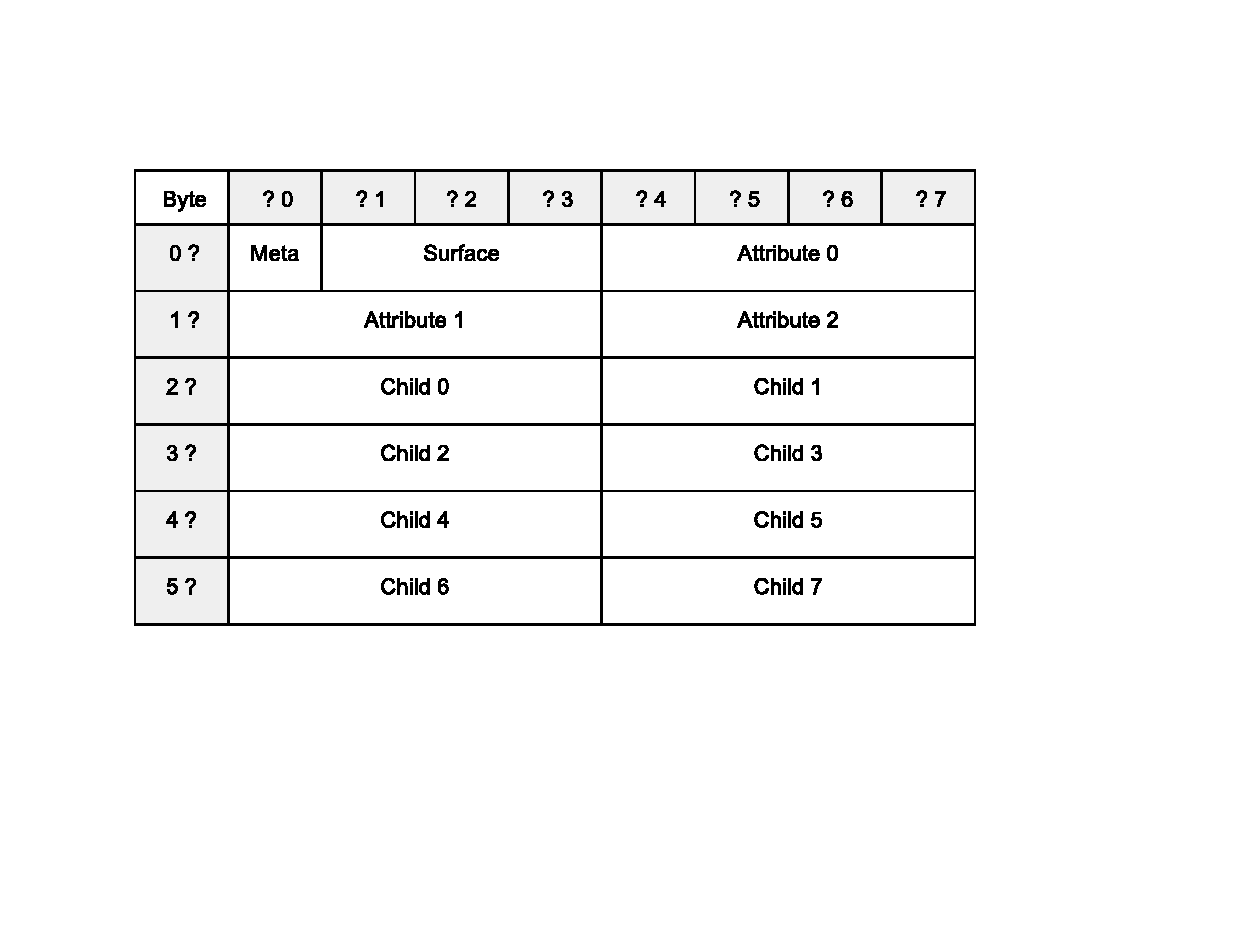
\includegraphics[width=\textwidth, viewport=50 120 475 380, clip=true]{nodeLayout.eps}
\caption{The data layout of a node. Byte positions are in octal for ease of representation.}
\end{center}
\end{figure}

The purpose of each of these fields is as follows:

\begin{itemize}

\item The meta value indicates the type of the voxel represented by a given node. This informs how data within each of the three attribute values are interpreted.
\item The surface value represents the normal of the surface represented by the voxel as well as the position of this surface within the voxel.
\item The attribute values, as stated previously, may be interpreted in a variety of ways depending upon the value of the meta value.
\item The child values are the offset of each child of the node in the data buffer, in units equal to the size of a node. Should the value of a child node be set to the maximum representable value for a 32-bit unsigned integer, this indicates that a child corresponding to this field does not exist. Considering such a node would theoretically be at the end of a buffer over 190 GB in size, which is well beyond the memory capacity of all current consumer graphics hardware, it is assumed such a node would not be created.
\end{itemize}


\foursection{The Head Buffer}

The Head Buffer is an array which stores the head node of each sparse voxel octree resident to the Voxel State. This buffer exists to provide a means of simply indexing into the head nodes of each SVO, which is a necessary initial operation for manipulating or tracing through an SVO.\\


\foursection{The Heap Buffer}

The Heap Buffer is where references to free nodes in the Data Buffer are stored for retrieval by Yggdrasil as need for more memory arises. The Heap Buffer houses an array of integers, grouped into sets of four, with a number of sets equivalent to the number of processor units present on the GPU. When a process from Yggdrasil intending to manipulate the Voxel State runs on the GPU, it must necessarily be the only manipulating process running on the GPU at the time. This is because each work item run during these jobs uses its global identification number to determine which of these sets of integers to use in order to get free memory. See figure 2 for diagram.

\begin{figure}[H]
\begin{center}
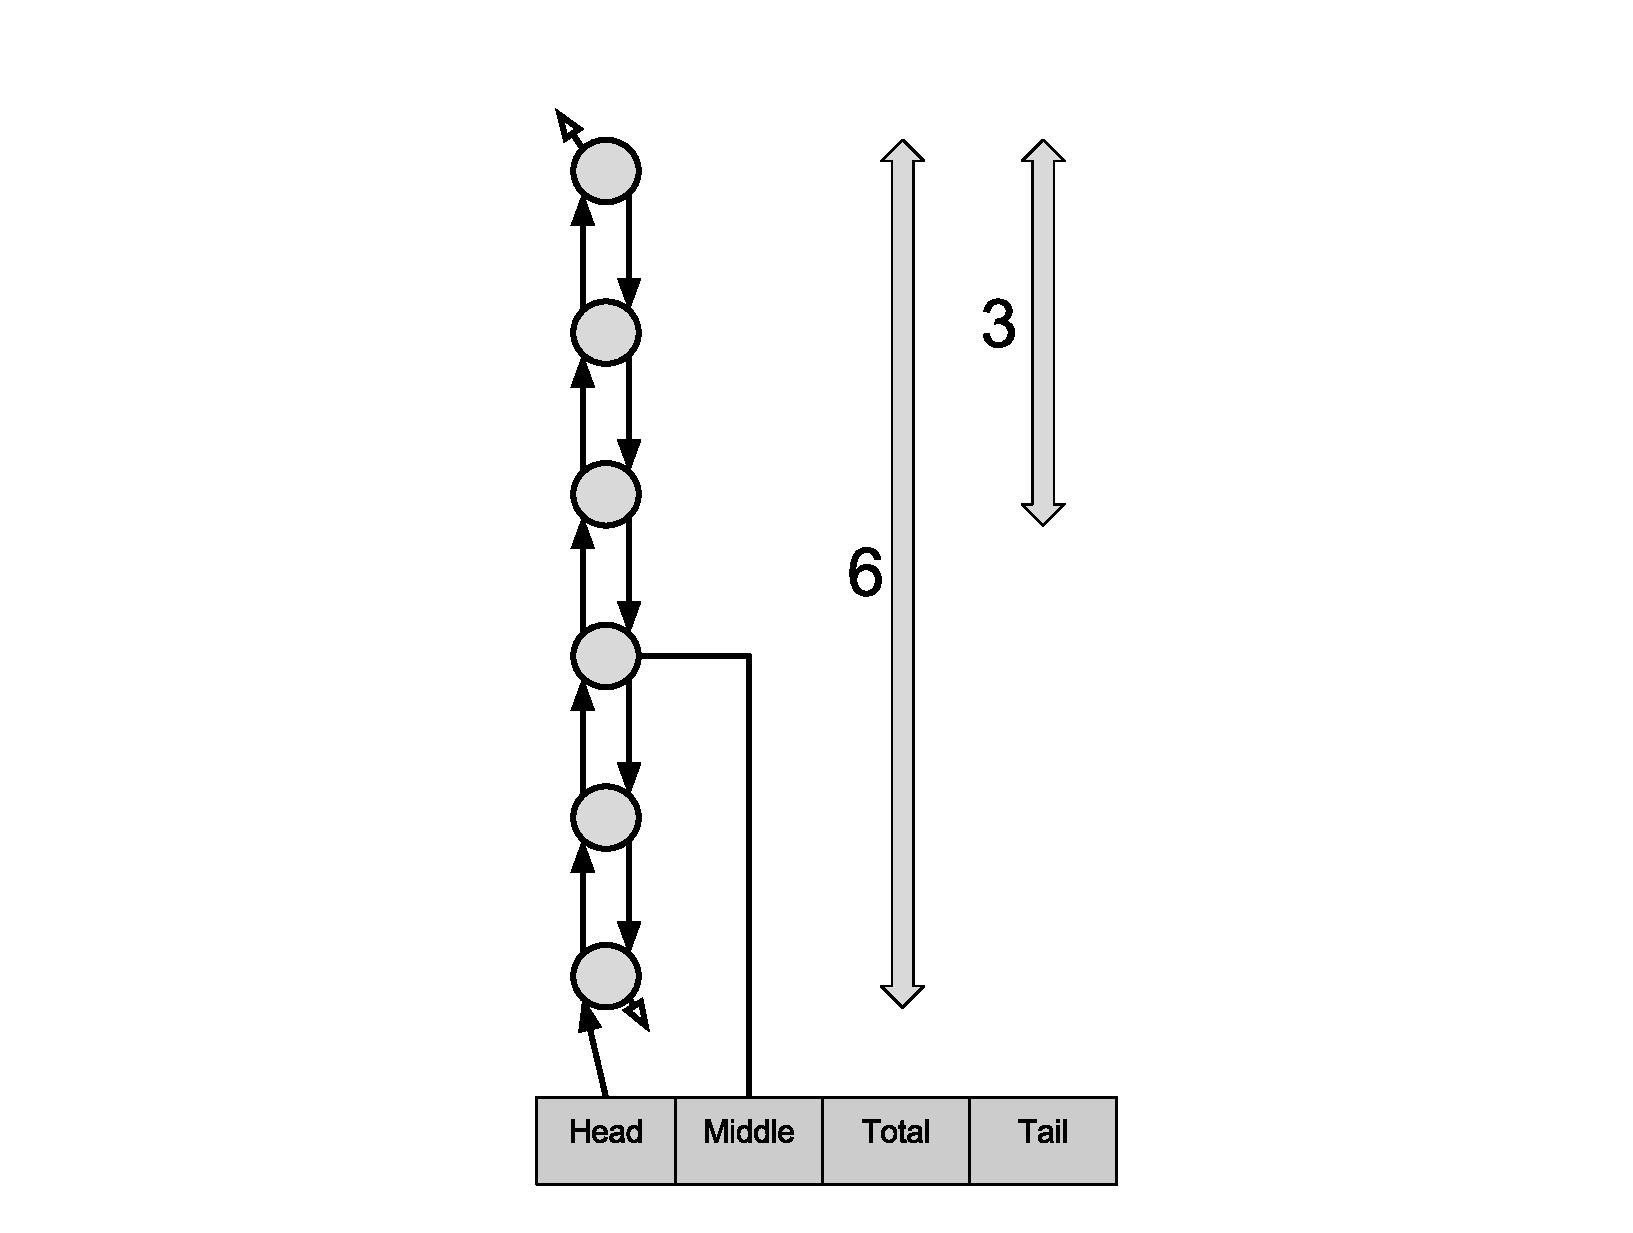
\includegraphics[width=\textwidth]{HeapBufferElement.eps}
\caption{The structure and nature of an element of the Heap Buffer}
\end{center}
\end{figure}

The first integer of these groups is the index of a node not used in the Data Buffer. This node forms the head of a linked list of other nodes, with each node using the child 0 and child 1 fields of each node to link it to its headward and tailward neighbors. Should the work unit corresponding to this triplet be in need of a free node, it retrieves the node from this index.

The second integer of these groups is the index of a node roughly in the center of the linked list indexed by the first integer. This is done for list balancing, which is discussed in the Yggdrasil section.

The third integer indicates the number of links in the list pointed to by the first integer, whereas the fourth integer indicates the number of links following the link indexed by the second integer. These are also used for list balancing.

When properly managed by Yggdrasil, the Heap Buffer provides constant-time access to each thread in the GPU and with no fragmentation among allocated memory, since allocating one node simply costs one nodes worth of memory. This means that not only is adding and removing items from the octree quick regardless of how much memory is being used, but only the memory that is needed is allocated from the Data Buffer.

\threesection{Components of the graphics engine (Yggdrasil)}

Yggdrasil, named for the cosmic world tree of Norse mythology, is the framework of GPU-native programs that are in charge of managing and rendering the Voxel State for PolyVox. As with the Voxel State, efficiency of memory usage as well as speed are strong design concerns. For this reason, reducing function runtime per input as well as memory footprint required for operations is key.

\foursection{The Data Buffer}
The Data Buffer holds all of the nodes that PolyVox uses to represent the voxels being viewed and interacted with by the user. Yggdrasil uses the position of a node in the Data Buffer when referencing it during Yggdrasil’s regular operation.
\foursection{The Head Buffer}
The Head Buffer is an array holding the index of the root of all SVOs present in the Data Buffer. This is used to uniquely identify every SVO in the Voxel State and is used at the beginning of each operation to begin tree traversals.
\foursection{The Heap Buffer}
The Heap Buffer is an array holding references to the heads of a series of linked lists composed of nodes. Additionally, next to each list reference is a reference to a link somewhere in the middle of the list, the number of links in the list, and the number of links between the second reference and the tail. This additional data is used to keep the length of the lists in the Heap Buffer close to one another, ensuring heavily used lists do not quickly run out of links.
\foursection{The Tool Executer}
The Tool Executer is a general-purpose OpenCL program template for the application of arbitrary operations to the Voxel State according to the user’s brush strokes and the currently selected tool. Whenever a new tool is loaded into PolyVox by the Interchange, the OpenCL code specific to that tool is injected into the template, which is then compiled into a tool executer. Regardless of what code is injected, much of the operation of the tool executer is the same.

The Tool Executer is passed a number of inputs based off the state of the brush stroke being performed by the user. This state includes what part of the stroke (beginning, middle, end) the operation is in, the line segment representing the path the stroke just made, the selected height, width, and depth of the brush tip used, the weight of the stroke, and the speed of the stroke.

Based on of the dimensions of the brush tip as well as the line segment representing the section of brush stroke just made, the Tool Executer traverses the SVO being actively edited, finding the smallest voxel in the octree which completely contains the bounds of the stroke section. Once this voxel is found, the voxel is given to the first section of injected tool code, which determines how much further the Tool Executer traverses into the octee. The code may either report that no more traversal is needed, or request further traversal. This request will be refused if the maximum resolution depth has been reached. If not, the Tool Executer allocates and attaches any missing child nodes, if necessary, then traverses into the nodes. This process is repeated until all traversals have reached bottom.

Once all Tool Executer traversals have reached their final depth, the voxels at the end of each trace are handed to a different set of injected code, which evaluates what the new state of each voxel should be. Once the new states are assigned and the injected code passes back execution, the Tool Executer reverses its traversals, applying a third piece of injected code to each parent voxel, ensuring that each one has a high-level representation of its children.

Once all traversals have been reversed, the Tool Executer terminates.
\foursection{The Renderer}

The Renderer is the OpenGL program executed in order to create the imagery that appears to the user in their HMD. The Renderer receives a set of triangles from the Interchange corresponding to the bounds of the SVO volumes visible to the user. This means that SVOs which do not intersect with the near plane of the user’s vision would be represented as boxes. Those SVOs that do intersect with the user’s near plane of vision would be represented as boxes truncated along the user’s near plane of vision.

Each of the vertices are given their corresponding position in the SVO as well as the index in the Head Buffer where the head of the box’s corresponding SVO is stored. Using this data, the fragment shader traverses the SVO as a voxel cone trace. As this trace is performed, for any given voxel it traces through, it will trace through its child nodes instead if that voxel has a cross section in the view projection larger than the fragment. This trace is performed until the contribution of samples to the final value of the trace drops below the smallest nonzero value representable by the trace's alpha component. Once the final value for a trace has been rendered, it is used as the color value for the fragment corresponding to that trace.\\

\foursection{The Memory Manager}

The Memory Manager is an OpenCL program which serves two purposes. Firstly, it performs balancing operations upon the Heap Buffer, alleviating imbalances in how much memory is available to each work group. Secondly, it provides information regarding the availability of memory in PolyVox to the Interchange, allowing the Interchange to take necessary action, such as calling for more memory, culling excess detail, or providing a warning to the user. See figure 3 for diagram.



\begin{figure}[H]
\begin{center}
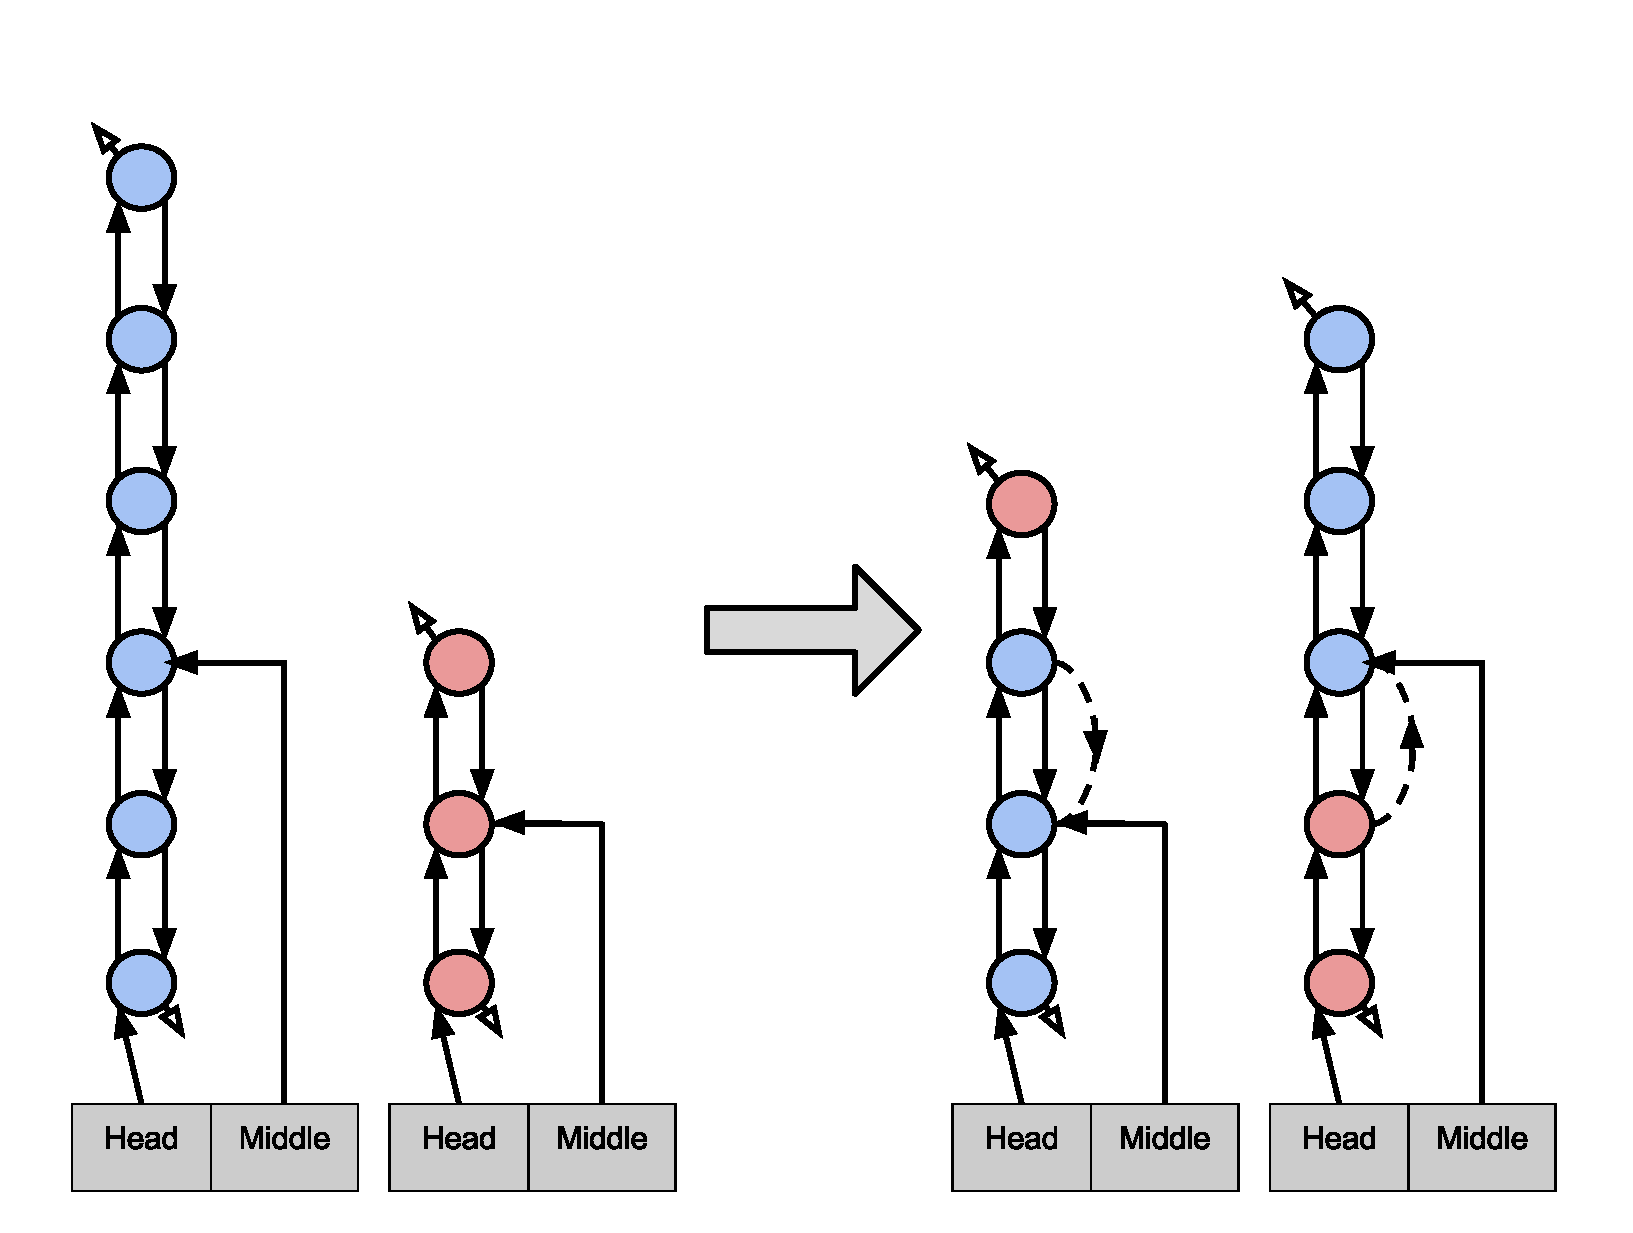
\includegraphics[width=\textwidth]{TailSwap.eps}
\caption{An example of a tail swap that could be carried out during a balancing procedure}
\end{center}
\end{figure}


The balancing procedure performed is relatively simple, each work item is given one of the linked lists. These work items then establish their position in a binary tree, where work items with a global id, n, have work items n*2 and n*2+1 as children. Work items at even depths in the tree inspect the data in its left child, retrieving the data member referencing a link in the middle of its linked list. Using this reference as well as the reference to a link in the middle of its own linked list, the acting working group switches the links across the two lists, causing all trailing links to also be appended to the other list. The link count members as well as the reference to the middle link for each work item are updated accordingly.

As stated previously, the middle links referenced for each linked list must be generally towards the center of the linked list. This is why the reference is traversed up or down the linked list up to sixteen links in order to begin approaching the halfway point for each list. This process is applied by the acting work groups to their right children, and these two processes are repeated by working groups at odd depths. Repeating this process multiple times, exchanging the tail half of each list, rebalancing halfway link references, then exchanging again, causes links to be more evenly distributed across the Heap Buffer.

Once these exchanges occur the number of times requested by the Interchange, the minimum and maximum linked list size is calculated through reduction and returned to the Interchange. This gives the Interchange a measure of how balanced the linked lists became as a result of the operation.

\threesection{Interactions between the hardware and the Interchange}
The VR HMD and motion controls act as the source of input for the user. The VR hardware will primarily interact with the system using pre-built drivers for the Unity engine, which are both easily available and open source. With such widely available device drivers, hardware implementation is, for the most part, a solved problem. The primary challenge from a design standpoint is how signals sent from, and received by the program are handled.

\foursection{Design Entities}
\textbf{Vive HMD} \\
The HTC Vive needs to have the HDMI, USB cable, and power adapter attached to the Vive's link box. The link box is then attached to the computer with an HDMI cable and USB cable. This completes the connection between the HMD and the computer.\\
\textbf{Vive Lighthouses} \\
The lighthouses and the integrated VR tracking solution need to be mounted on the wall or with stands. They must be connected to power and programmed to ‘A’ and ‘B’ channels within the VR driver. They must also have a BNC sync cable running between them. If the sync cable does not fit the volume model, then we must use channels ‘B’ and ‘C.’ The light houses must be spaced at least 15 feet apart. 
\foursection{Design} 
The driver is operated by the Steam VR asset in the Unity add-on window. The driver takes in input through the HMD and uses the data to manipulate the camera rig object in Unity. The Steam VR library allows for controller input to be passed to the game engine. This input must then be mapped to a trackable object in Unity. This object can then be used by the Interchange for processing. The same process is performed using data sent by the HMD. The packets sent by the controllers and HMD will be done through USB and sent to the Interchange. We will need position and orientation of the HMD and at least on of the Vive controllers. We will also need trackpad and trigger inputs from the controller. This will be sent to PolyVox and into the Interchange driver.

\threesection{Architecture of the User Interface}
The UI will essentially be a game object that can be moved and accessed around the peripheral of the user. The user should have the option to specify rotation lock, where the UI object follows them everywhere they look. This allows the user to have access to the toolset at all times. Turning this off will only invoke position lock, where the UI object is always at a relative position to the user. 

\foursection{Design Entities}
\textbf{Brush Object} \\
Brush objects will be game objects operated by the UI and the game engine. Each brush object contains position and orientation of a motion controller, as well as whatever graphical transformations will be applied when a modify geometry command is sent via a button press.

\foursection{Design}
The UI will have two initial states, active and inactive. The inactive UI will be a small game object only capable of a few actions. The user can turn on or off the rotation lock. The user can move the UI object to another relative position while in this state. The state also has a way of moving the UI into the active state. 
The active state will have all of the same features as the inactive state, except that it can invoke the inactive state instead of the active state. It also can navigate a tree structure that gives the user access to all of the tools and environment settings. 

The UI response to track pad inputs on the Vive controller as well as the track pad target position. The trackpad press event. This acts as a confirmation operation when toggling states or selecting items in the UI. The UI will be structured to take advantage of non physical position dependence by allowing the trackpad to operate independently of the controller's physical position and orientation. This allows the user to operate the UI in the world space without relying on VR tracking.

The active UI design needs to be full capable of accessing all of the features in its layout. The layout will always have a button at the top for moving backwards. When at the top layer, this button moves from active to inactive. Each item in the UI will either be a UI element or a traversal node. The traversal nodes allow separation of UI pages and access to other nodes. The UI elements are access to settings and tools. UI elements can be things like brush type or brush color. See figure 4 for diagram.

\begin{figure}[H]
\begin{center}
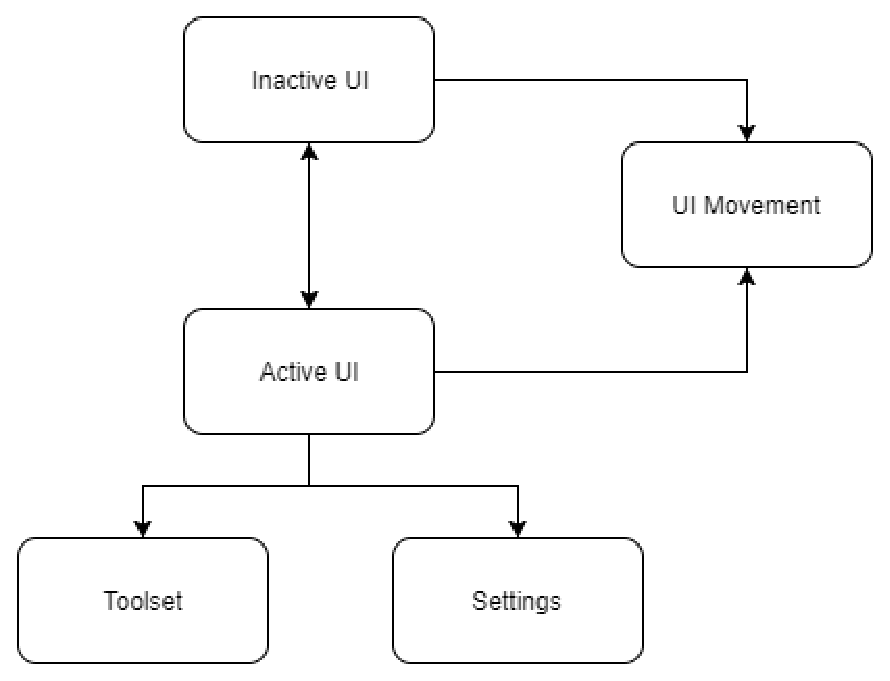
\includegraphics[width=\textwidth]{UIDiagram.eps}
\caption{An example of a tail swap that could be carried out during a balancing procedure}
\end{center}
\end{figure}

\threesection{Architecture of the Interchange}
The Interchange will be the primary point of communication and manager for the disparate elements of the program. The Interchange must be able to receive information supplied via the user interface and interface hardware and relay the corresponding instruction to the Yggdrasil engine to properly render the scene, and is directly responsible for directing state transition of all other components. Due to the experimental nature of the project, the design of the Interchange must be kept at a high level. Specifics of functions and the processing of data will need to be determined in development. 

The Interchange must be capable of properly coordinating all other elements of PolyVox as a whole, and is a central element  in executing commands supplied via user interactions, implementing program features, and directing the graphics engine’s rendering operations. As such it is relevant to design concerns of all stakeholders involved in the project. In particular, it is central to the operation of the user interface and motion controls, from which it will receive user commands, and the operation of the graphics engine, which it will send commands to. As the Interchange will be the point at which the program’s toolset is constructed, it will also dictate the program’s available features.

\foursection{Design Entities}
\textbf{Unity Engine:}\\
The Interchange will be built in and run on the Unity Game Engine. Unity has its own proprietary rendering and modeling systems, as well as native compatibility with motion tracking systems and dual rendering used in VR. Additionally, Unity has native scripting compatibility and will serve as the platform for developing the program tools and features.\cite{unity}\\
\textbf{C\#:}\\
C\# is one of the most frequently used languages for scripting in game engines, and is natively compatible with Unity. Most features and tools for the program will be constructed using C\#. 

\foursection{Design}
When in operation, the Interchange will receive positional information from the user via both the HMD and VR motion controls in the form of four-element vector positional coordinates. Using Unity’s native VR drivers, the Interchange will translate these coordinates into a position relative to the voxel state.

Additionally, the data received from the user may or may not include a user-inputted command via a button press. When pressed, the button input will be sent to a function, which is also passed the current state of the UI (such as what ‘brush’ is selected, or what menu the user currently has open). The function will process the user command to determine any possible UI state changes, as well as any changes to the voxel state the user command will perform (such as creating or destroying a voxel) based on whatever tool or UI element is currently being operated. 

Any changes in the state are returned by the function as a set of commands to the graphics engine. The graphics engine will then process the commands from the Interchange. Before the render is sent to the HMD, the graphics engine will return a flag that will determine if the Interchange needs to perform additional actions, such as sending a command to the GPU to allocate additional memory. If so, the Interchange will send the appropriate commands, and the graphics engine will reattempt the render. This repeats until the flag sent from the GPU is null. 

While the operations of the Interchange are primarily just in service to other elements of the program, they are still vitally necessary to PolyVox’s operation. The Interchange effectively acts as the driver for the graphics engine and the motion control system, and is needed in order to develop a working feature set and comfortable user interface. See figure 5 for diagram.

\begin{figure}[H]
\begin{center}
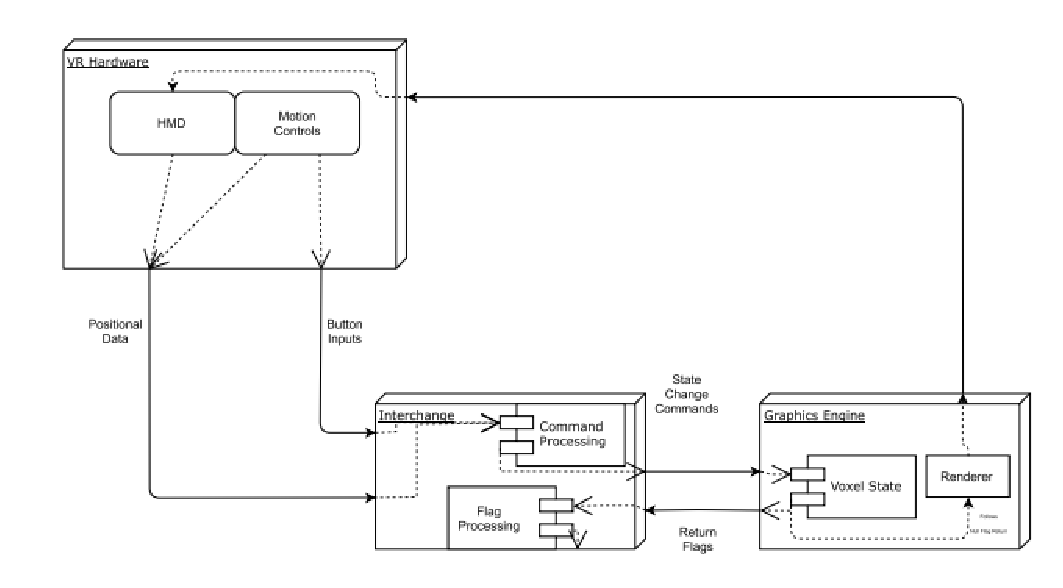
\includegraphics[width=\textwidth]{Interchange.eps}
\caption{General architecture of the Interchange}
\end{center}
\end{figure}


\subsection{Amendments}

\subsection{Gantt Chart}



\section{Design Document}

\subsection{Original Document}

\subsection{Amendments}



\section{Technology Review}





\section{Weekly Blog Posts}




\section{Final Poster}




\section{Project Documentation}

\subsection{Theory of Operation}



\subsection{System Requirements}


\subsection{Installation Process}


\subsection{Usage Guide}



\section{Recommended Technical Resources for Learning More}




\section{Conclusions and Reflections}


\subsection{Christopher Bakkom}

\subsubsection{Technical Information Learned}
What technical information did I learn
\subsubsection{Non-Technical Information Learned}
What non-technical information did I learn?
\subsubsection{Project Work Skills Learned}
What have I learned about project work?
\subsubsection{Project Management Skills Learned}
What have I learned about project management?
\subsubsection{Teamwork Skills Learned}
What have I learned about working in teams?
\subsubsection{Reflection}
If I could do it all over, what would I do differently?


\subsection{Richard Cunard}

\subsubsection{Technical Information Learned}
What technical information did I learn
\subsubsection{Non-Technical Information Learned}
What non-technical information did I learn?
\subsubsection{Project Work Skills Learned}
What have I learned about project work?
\subsubsection{Project Management Skills Learned}
What have I learned about project management?
\subsubsection{Teamwork Skills Learned}
What have I learned about working in teams?
\subsubsection{Reflection}
If I could do it all over, what would I do differently?


\subsection{Braxton Cuneo}

\subsubsection{Technical Information Learned}
What technical information did I learn
\subsubsection{Non-Technical Information Learned}
What non-technical information did I learn?
\subsubsection{Project Work Skills Learned}
What have I learned about project work?
\subsubsection{Project Management Skills Learned}
What have I learned about project management?
\subsubsection{Teamwork Skills Learned}
What have I learned about working in teams?
\subsubsection{Reflection}
If I could do it all over, what would I do differently?


\appendix

\section{Appendix 1: Essential Code Listings}

\section{Appendix 2: Additional Media}


\end{document}
